%!TEX root = ../thesis.tex


\begin{table}[]
\centering
\resizebox{\linewidth}{!}{%
\begin{tabularx}{\textwidth}{|l|X|}
\hline
Method                & Description \\ \hline
execCommand           & Executes a command. \\ \hline
queryCommandEnabled   & Returns whether or not a given command can currently be executed. \\ \hline
queryCommandIndeterm  & Returns whether or not a given command is in the indeterminate state. \\ \hline
queryCommandState     & Returns the current state of a given command. \\ \hline
queryCommandSupported & Returns whether or not a given command is supported by the current document's range. \\ \hline
queryCommandValue     & Returns the value for the given command. \\ \hline
\end{tabularx}
}
\caption{HTML Editing API}
\label{table:editing_mode_api}
\end{table}


\clearpage
\newpage

%\begin{landscape}


%%%%%%%%%%%%%%%%%%%%%%%
\begin{table}[]
\centering
\resizebox{\linewidth}{!}{%
\begin{tabularx}{\textwidth}{|l|X|}
\hline
Example call    &    Description \\ \hline

type.caret()	&	 Returns the offset of the caret. \\ \hline
type.caret('show')	&	 Shows the caret. \\ \hline
type.caret('hide')	&	 Hides the caret. \\ \hline
type.caret(10)	&	 Moves the caret to the 10th character. \\ \hline
type.caret(10, 20)	&	 Convenience function for type.select(10, 20). \\ \hline

\end{tabularx}
}
\caption{Type instance API: caret command}
\label{table:instance_api_caret_command}
\end{table}

%%%%%%%%%%%%%%%%%%%%%%%

\begin{table}[]
\centering
\resizebox{\linewidth}{!}{%
\begin{tabularx}{\textwidth}{|l|X|}
\hline
Example call    &    Description \\ \hline

type.selection()	&	 Same as type.selection('html'). \\ \hline
type.selection('text')	&	 Returns the unformatted (plain) contents of the current selection. \\ \hline
type.selection('html')	&	 Return the currently selected HTML. \\ \hline
type.selection(10)	&	 Convenience function for type.caret(10). \\ \hline
type.selection(10, 20)	&	 Selects characters 10 to 20. \\ \hline
type.selection(element)	&	 Select an element. \\ \hline
type.selection(el1, el2)	&	 Creates a selection between 2 elements. \\ \hline
type.selection(jQuery obj.)	&	 Creates a selection between the first and last element in a jQuery object. \\ \hline
type.selection('save')	&	 Returns an object that can be passed to type.selection('restore') to store and recreate a selection. \\ \hline
type.selection('restore', sel)	&	 Takes an object returned by type.selection('save') as a second argument to recreate a stored selection. \\ \hline

\end{tabularx}
}
\caption{Type instance API: selection command}
\label{table:instance_api_selection_command}
\end{table}

%%%%%%%%%%%%%%%%%%%%%%%

\begin{table}[]
\centering
\resizebox{\linewidth}{!}{%
\begin{tabularx}{\textwidth}{|l|X|}
\hline
Example call    &    Description \\ \hline

type.insert(str)	&	 Inserts formatted text at the caret's position. Will overwrite the current	 selection if there is one. \\  \hline
type.insert(str, 'text')	&	 Inserts plain text at the caret's position removing all formattings from str. Will overwrite the current selection if there is one. \\ \hline
type.insert(str, 10)	&	 Inserts str after the 10th character in the text. \\ \hline
type.insert(str, 10, 'text')	&	 Same as type.insert(str, 10) but inserts unformatted text. \\ \hline

\end{tabularx}
}
\caption{Type instance API: insert command}
\label{table:instance_api_insert_command}
\end{table}

%%%%%%%%%%%%%%%%%%%%%%%

\iffalse
%\begin{table}[]
\centering
\resizebox{\linewidth}{!}{%
\begin{tabularx}{\textwidth}{|l|X|}
\hline
Example call    &    Description \\ \hline

type.replace(str, 10, 20)	&	 Replaces text between offset 10 and 20 with the text given as str \\ \hline
type.replace('html', str, 10, 20)	&	 Same as type.replace(str, 10, 20) but inserts formatted text given as html string \\ \hline

\end{tabularx}
}
\caption{Type instance API: replace command}
\label{table:instance_api_replace_command}
%\end{table}
\fi

%%%%%%%%%%%%%%%%%%%%%%%

\begin{table}[]
\centering
\resizebox{\linewidth}{!}{%
\begin{tabularx}{\textwidth}{|l|X|}
\hline
Example call    &    Description \\ \hline

type.format(htmlString)    &    Formats the currently selected text with the markup passed as htmlString. \\ \hline
type.format(htmlString, 10, 20)    &    Formats the characters 10 to 20 in the text with the markup passed as htmlString. \\ \hline

%type.format(tagName, [...params])	&	 Formats the currently selected text with the given tag. E.g. use type.cmd('strong') to format the currently selected text bold \\ \hline
%type.format(startOffset, endOffset, tagName, [...params])	&	 Applies type.format to a specific text range \\ \hline

\end{tabularx}
}
\caption{Type instance API: format command}
\label{table:instance_api_format_command}
\end{table}

%%%%%%%%%%%%%%%%%%%%%%%

\begin{table}[]
\centering
\resizebox{\linewidth}{!}{%
\begin{tabularx}{\textwidth}{|l|X|}
\hline
Example call    &    Description \\ \hline

type.remove()	&	 Deletes the currently selected text. Does nothing if there is no selection. \\ \hline
%type.remove(numChars)	&	 Removes a number of characters from the caret's position. A negative number will remove characters left of the caret, a positive number from the right. If there is a selection, the characters will be removed from the end of the selection. \\ \hline
type.remove(5)	&	 Removes 5 characters right of the caret's offset. Removes the first 5 characters of the selection if there is a text selection. \\ \hline
type.remove(-5)	&	 Removes 5 characters left of the caret's offset. Removes the last 5 characters of the selection if there is a text selection. \\ \hline
type.remove(10, 20)	&	 Will remove the text between the 10th and 20th character. \\ \hline

\end{tabularx}
}
\caption{Type instance API: remove command}
\label{table:instance_api_remove_command}
\end{table}

%%%%%%%%%%%%%%%%%%%%%%%

\begin{table}[]
\centering
\resizebox{\linewidth}{!}{%
\begin{tabularx}{\textwidth}{|l|X|}
\hline
Example call    &    Description \\ \hline

type.undo()	&	Revokes the user's last action.  \\ \hline
type.undo(5)	&	Revokes the user's last 5 actions.  \\ \hline
type.redo()	&	Reapplies a revoked action.  \\ \hline
type.redo(5)	&	Reapplies 5 revoked actions.  \\ \hline

\end{tabularx}
}
\caption{Type instance API: undo and redo commands}
\label{table:instance_api_undoredo_command}
\end{table}

%%%%%%%%%%%%%%%%%%%%%%%

\begin{table}[]
\centering
\resizebox{\linewidth}{!}{%
\begin{tabularx}{\textwidth}{|l|X|}
\hline
Example call    &    Description \\ \hline

type.options()	&	 Returns all settings of an instance. \\ \hline
type.options(name)	&	 Getter for a specific setting of an instance. \\ \hline
type.options(name, values)	&	 Setter for a specific setting of an instance. \\ \hline
type.options(\{name: value\})	&	 Pass an object to set multiple settings of an instance. \\ \hline

\end{tabularx}
}
\caption{Type instance API: options command}
\label{table:instance_api_options_command}
\end{table}

%\end{landscape}



\clearpage
\newpage

\begin{landscape}

  \begin{figure}[htb]
    \centerline{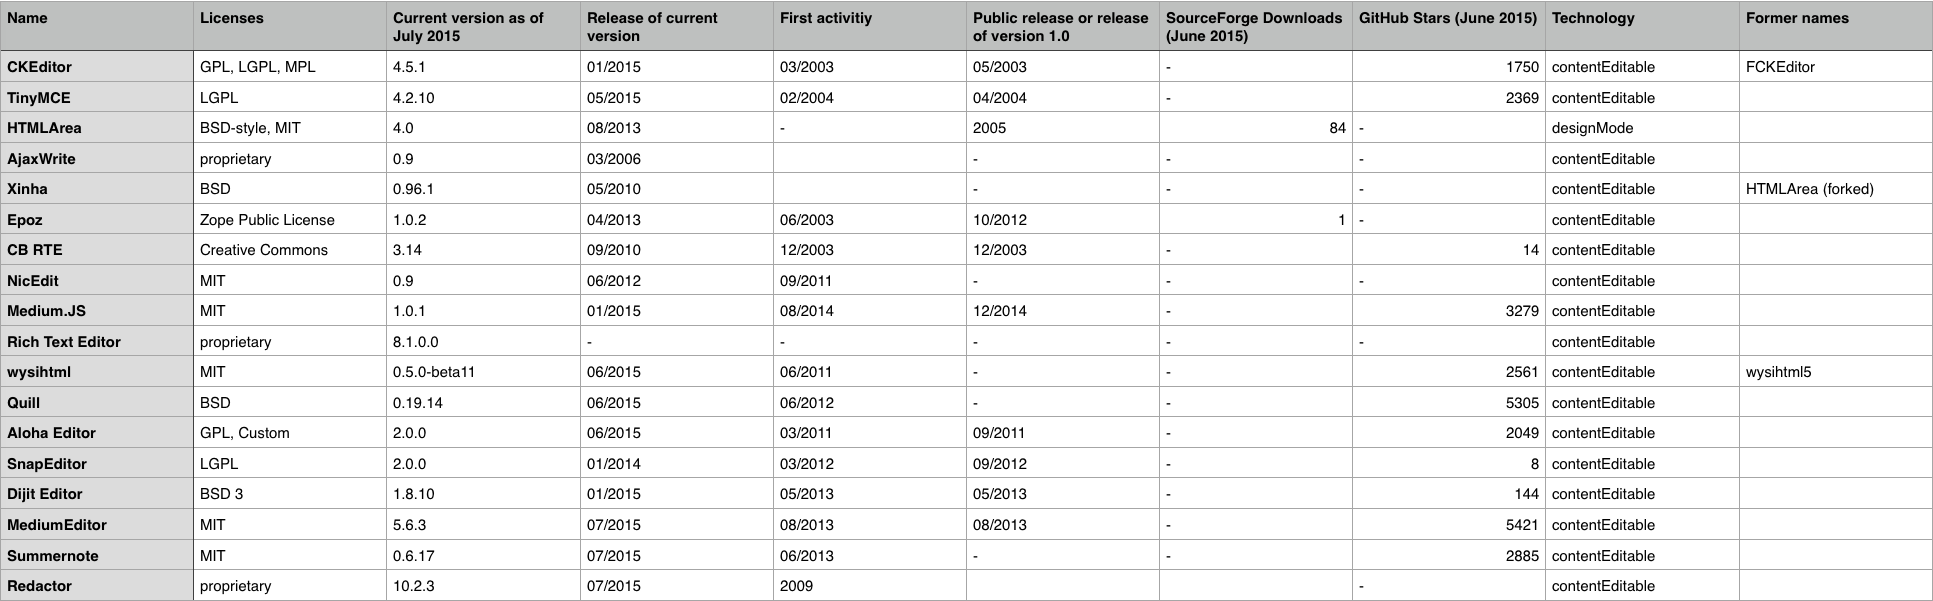
\includegraphics[width=\linewidth]{images/table-ce-editors.png}}
    \caption{Editors using HTML editing APIs (selection)}
    \label{fig:editors_editing_apis_table}
  \end{figure}
  
  \begin{figure}[htb]
    \centerline{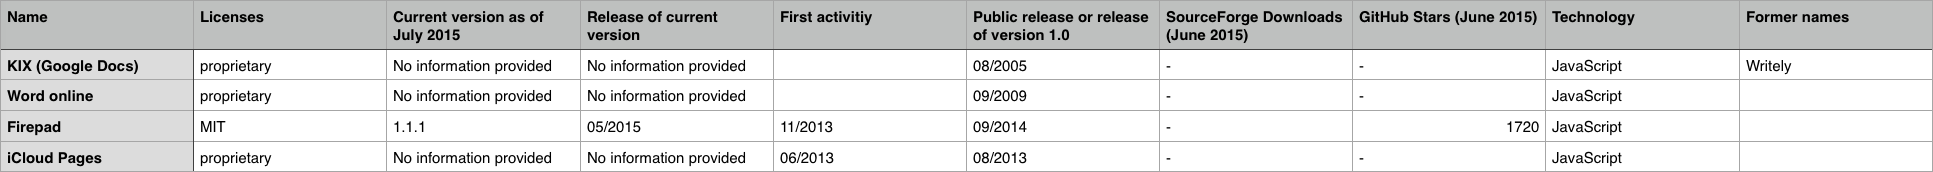
\includegraphics[width=\linewidth]{images/table-js-editors.png}}
    \caption{Editors not using HTML editing APIs (selection)}
    \label{fig:editors_not_editing_apis_table}
  \end{figure}
  
\end{landscape}


\clearpage
\newpage

\begin{landscape}
  \begin{figure}[htb]
    \centerline{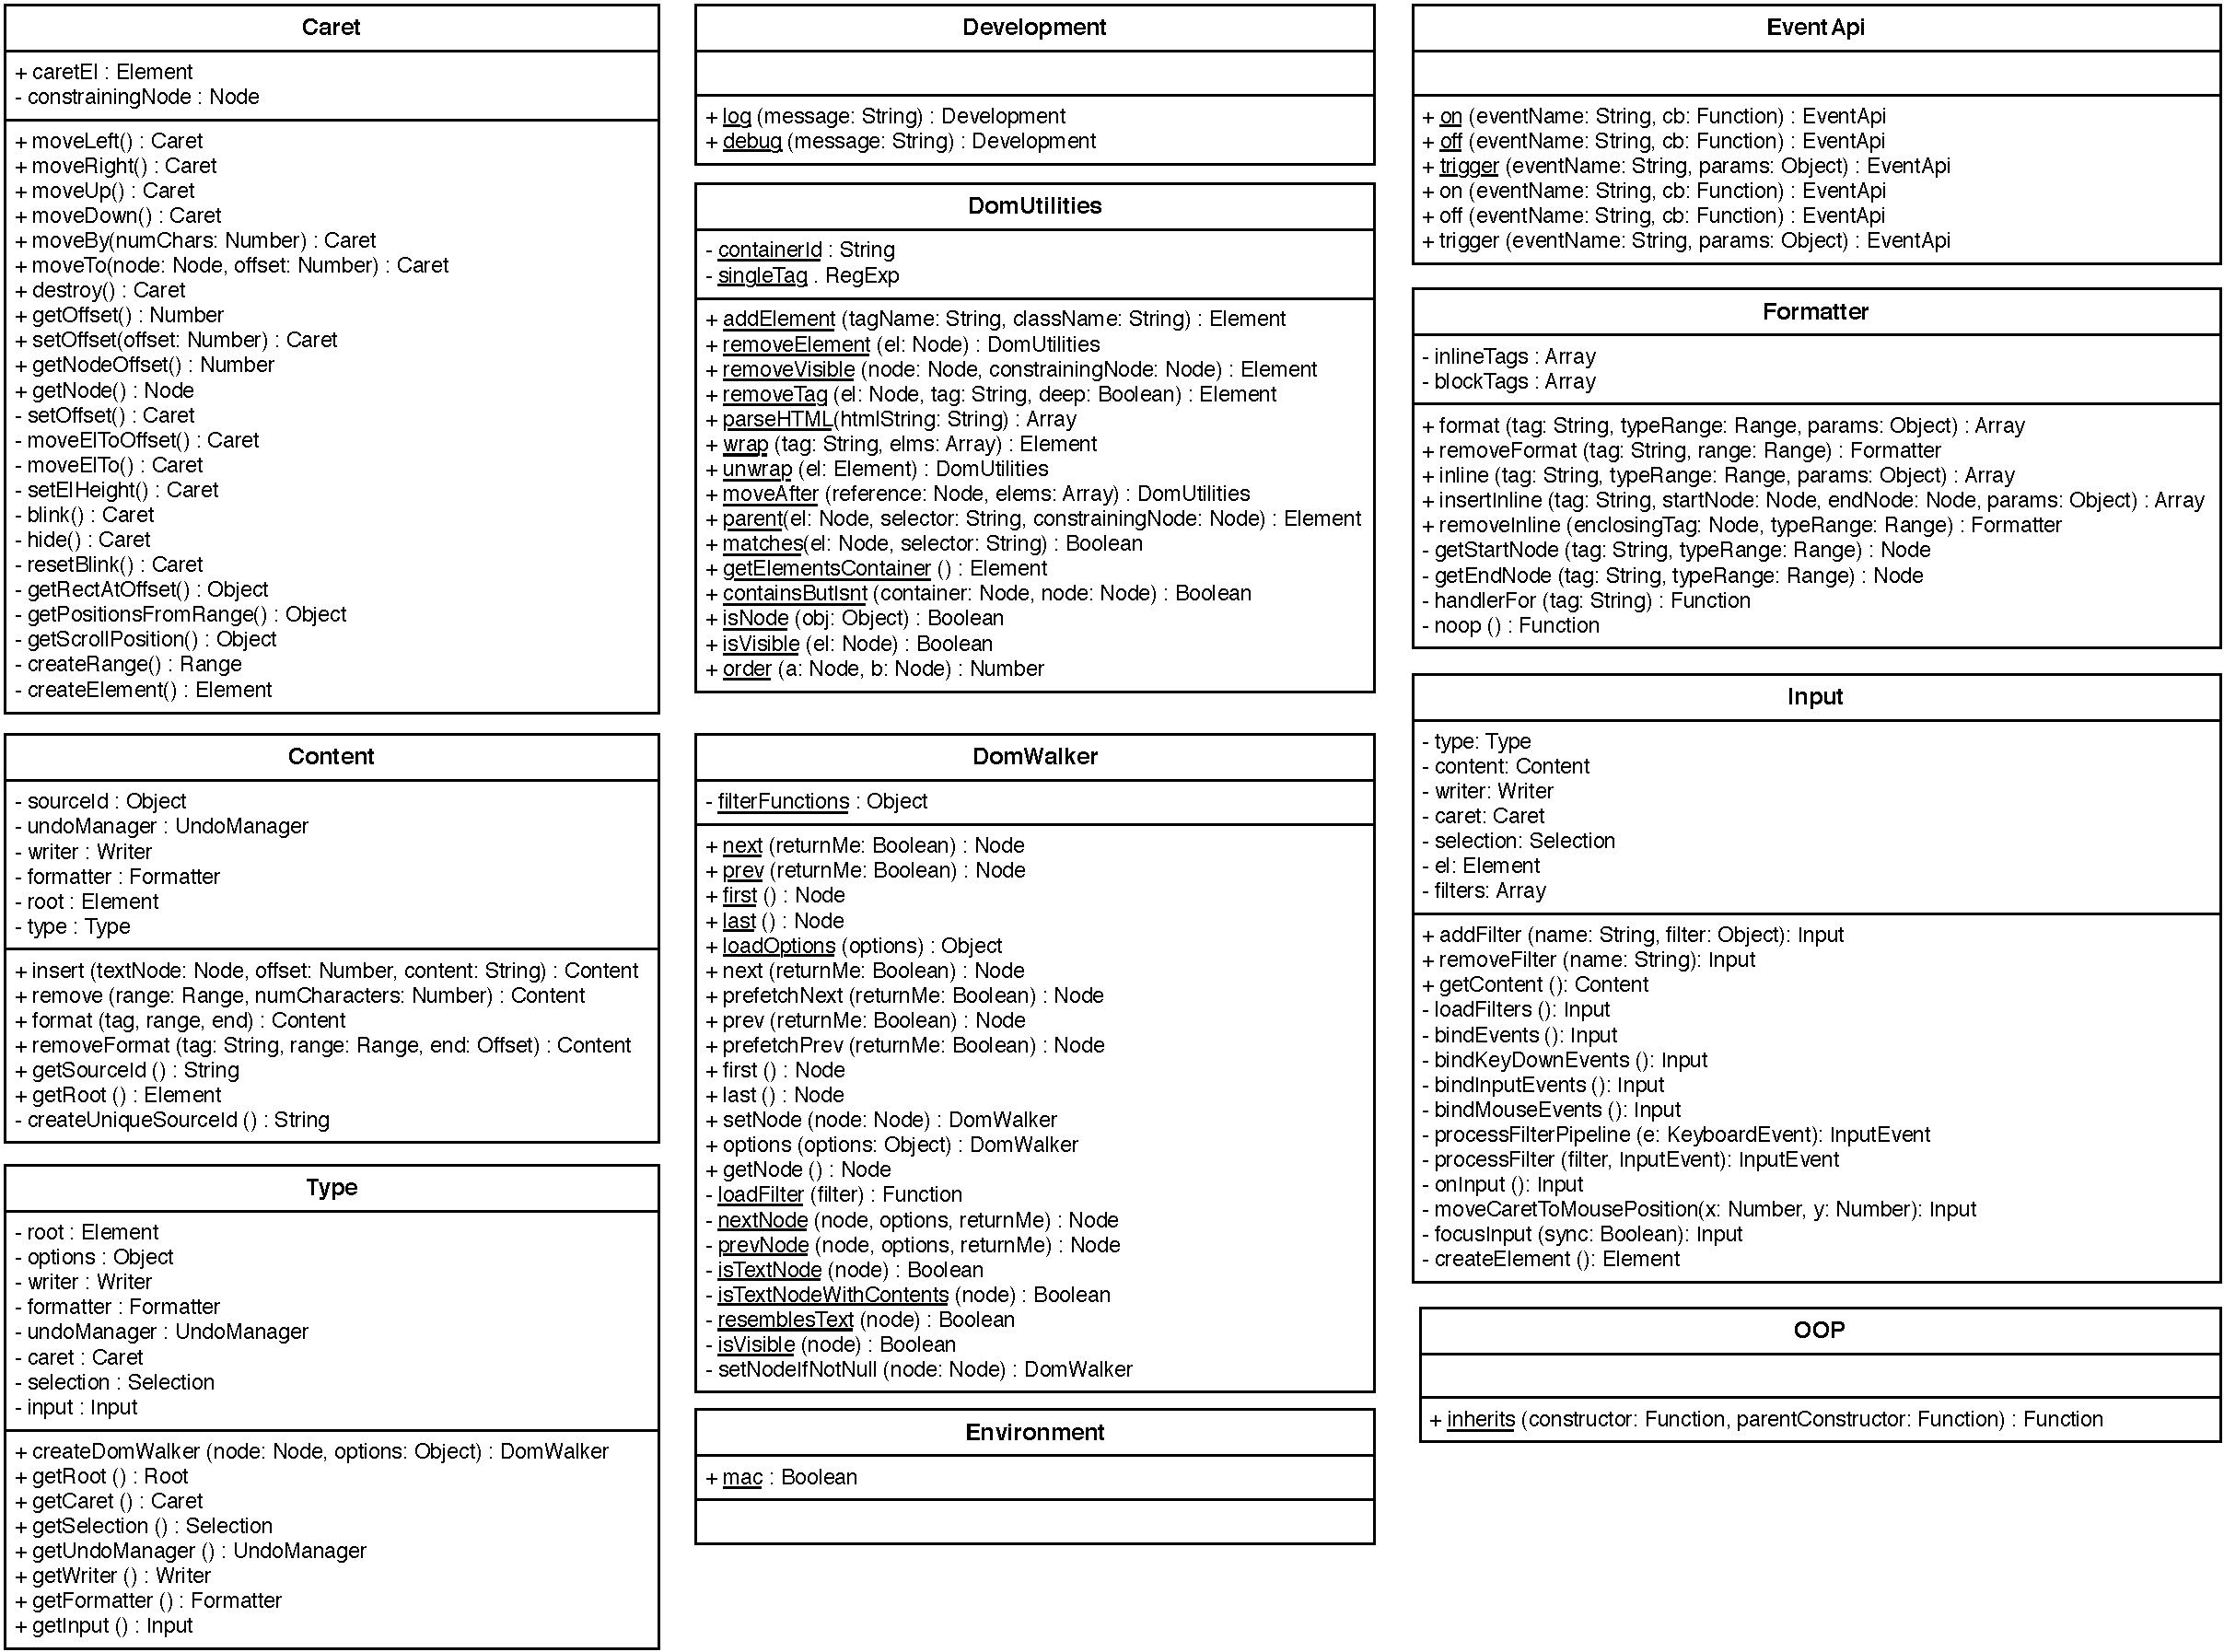
\includegraphics[width=.9\linewidth]{images/ClassesType-1}}
    \caption{Classes of the library 1/3}
    \label{fig:classes_type_one}
  \end{figure}
\end{landscape}

\clearpage
\newpage

\begin{landscape}
  \begin{figure}[htb]
    \centerline{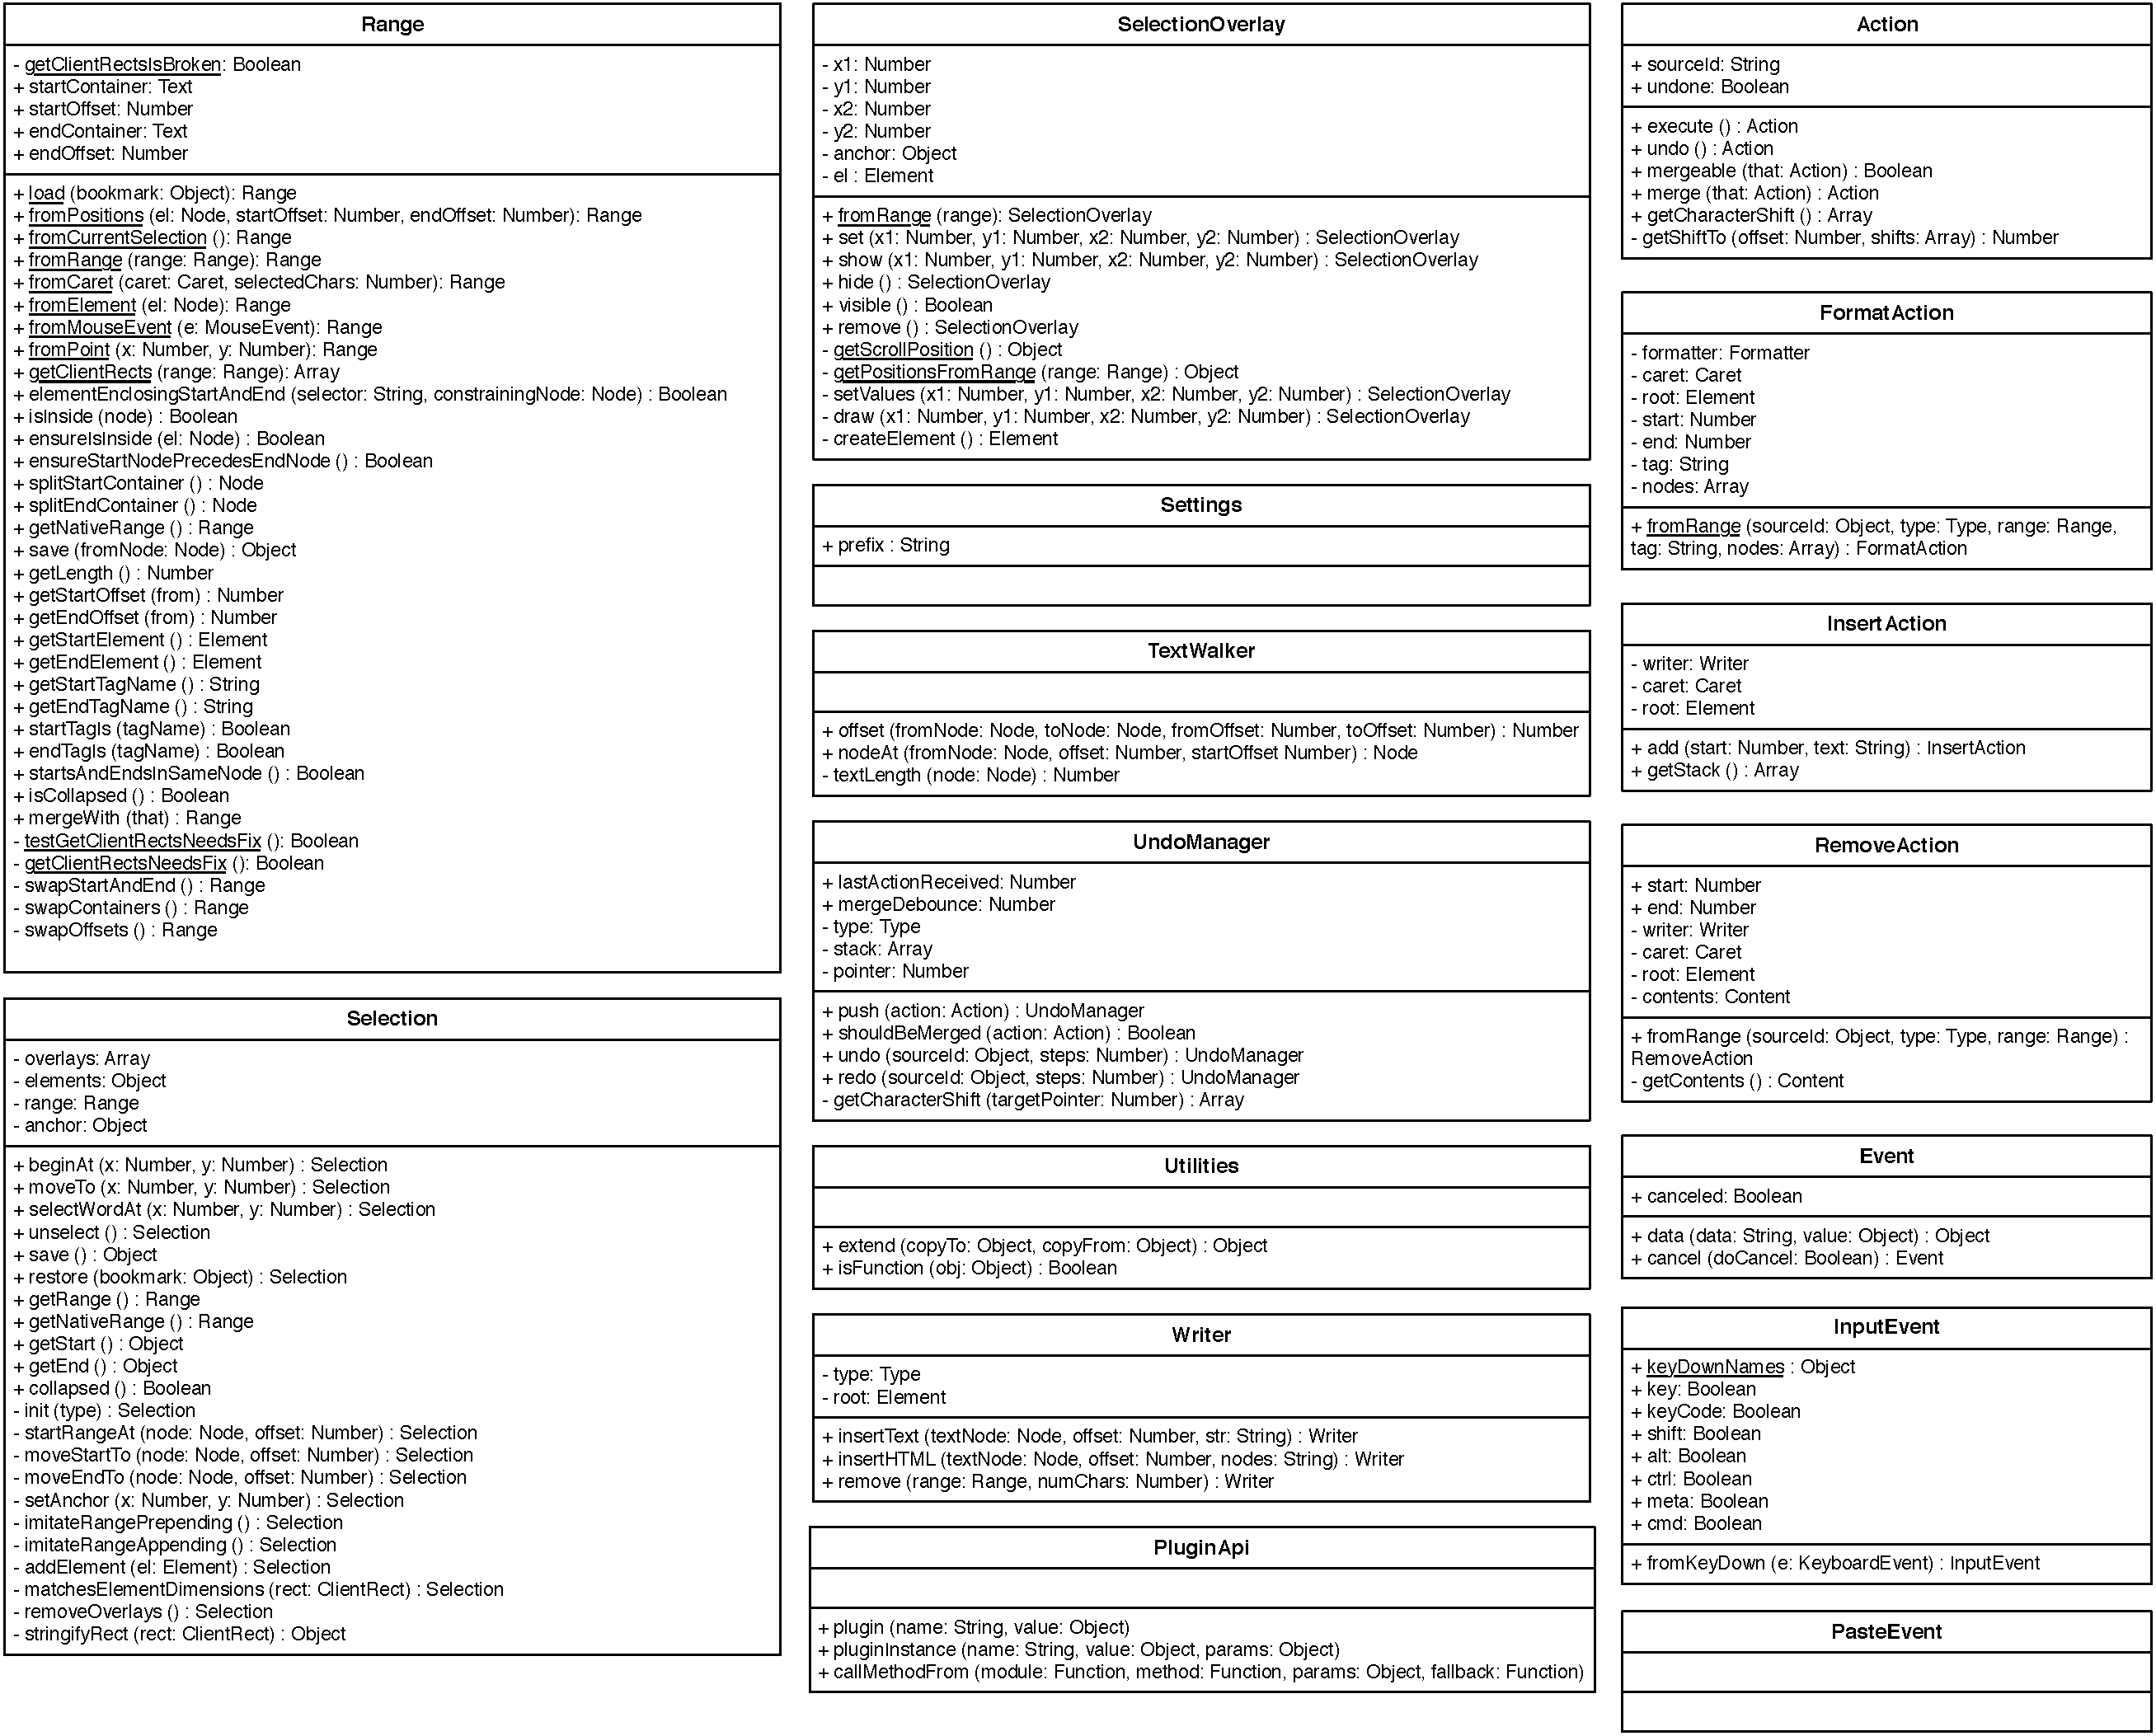
\includegraphics[width=.75\linewidth]{images/ClassesType-2}}
    \caption{Classes of the library 2/3}
    \label{fig:classes_type_two}
  \end{figure}
\end{landscape}

\clearpage
\newpage

\begin{landscape}
  \begin{figure}[htb]
    \centerline{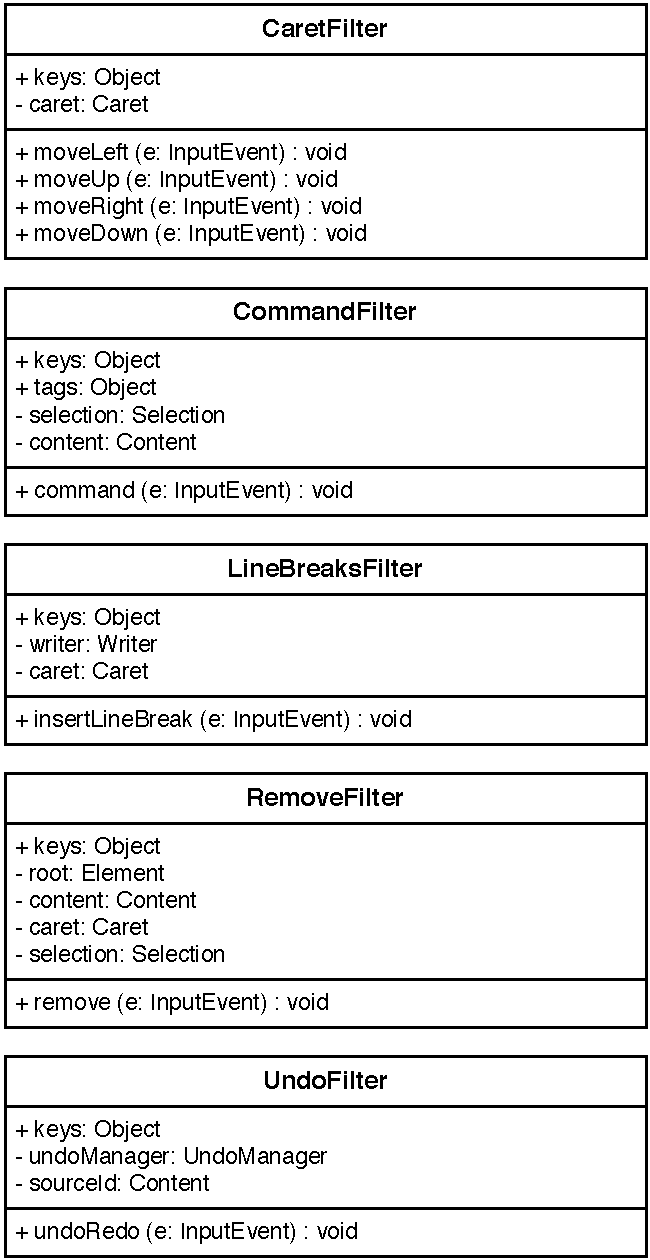
\includegraphics[width=\textwidth,height=\textheight,keepaspectratio]{images/ClassesType-3}}
    \caption{Classes of the library 3/3}
    \label{fig:classes_type_three}
  \end{figure}
\end{landscape}

\clearpage
\newpage

\begin{landscape}
  \begin{figure}[htb]
    \centerline{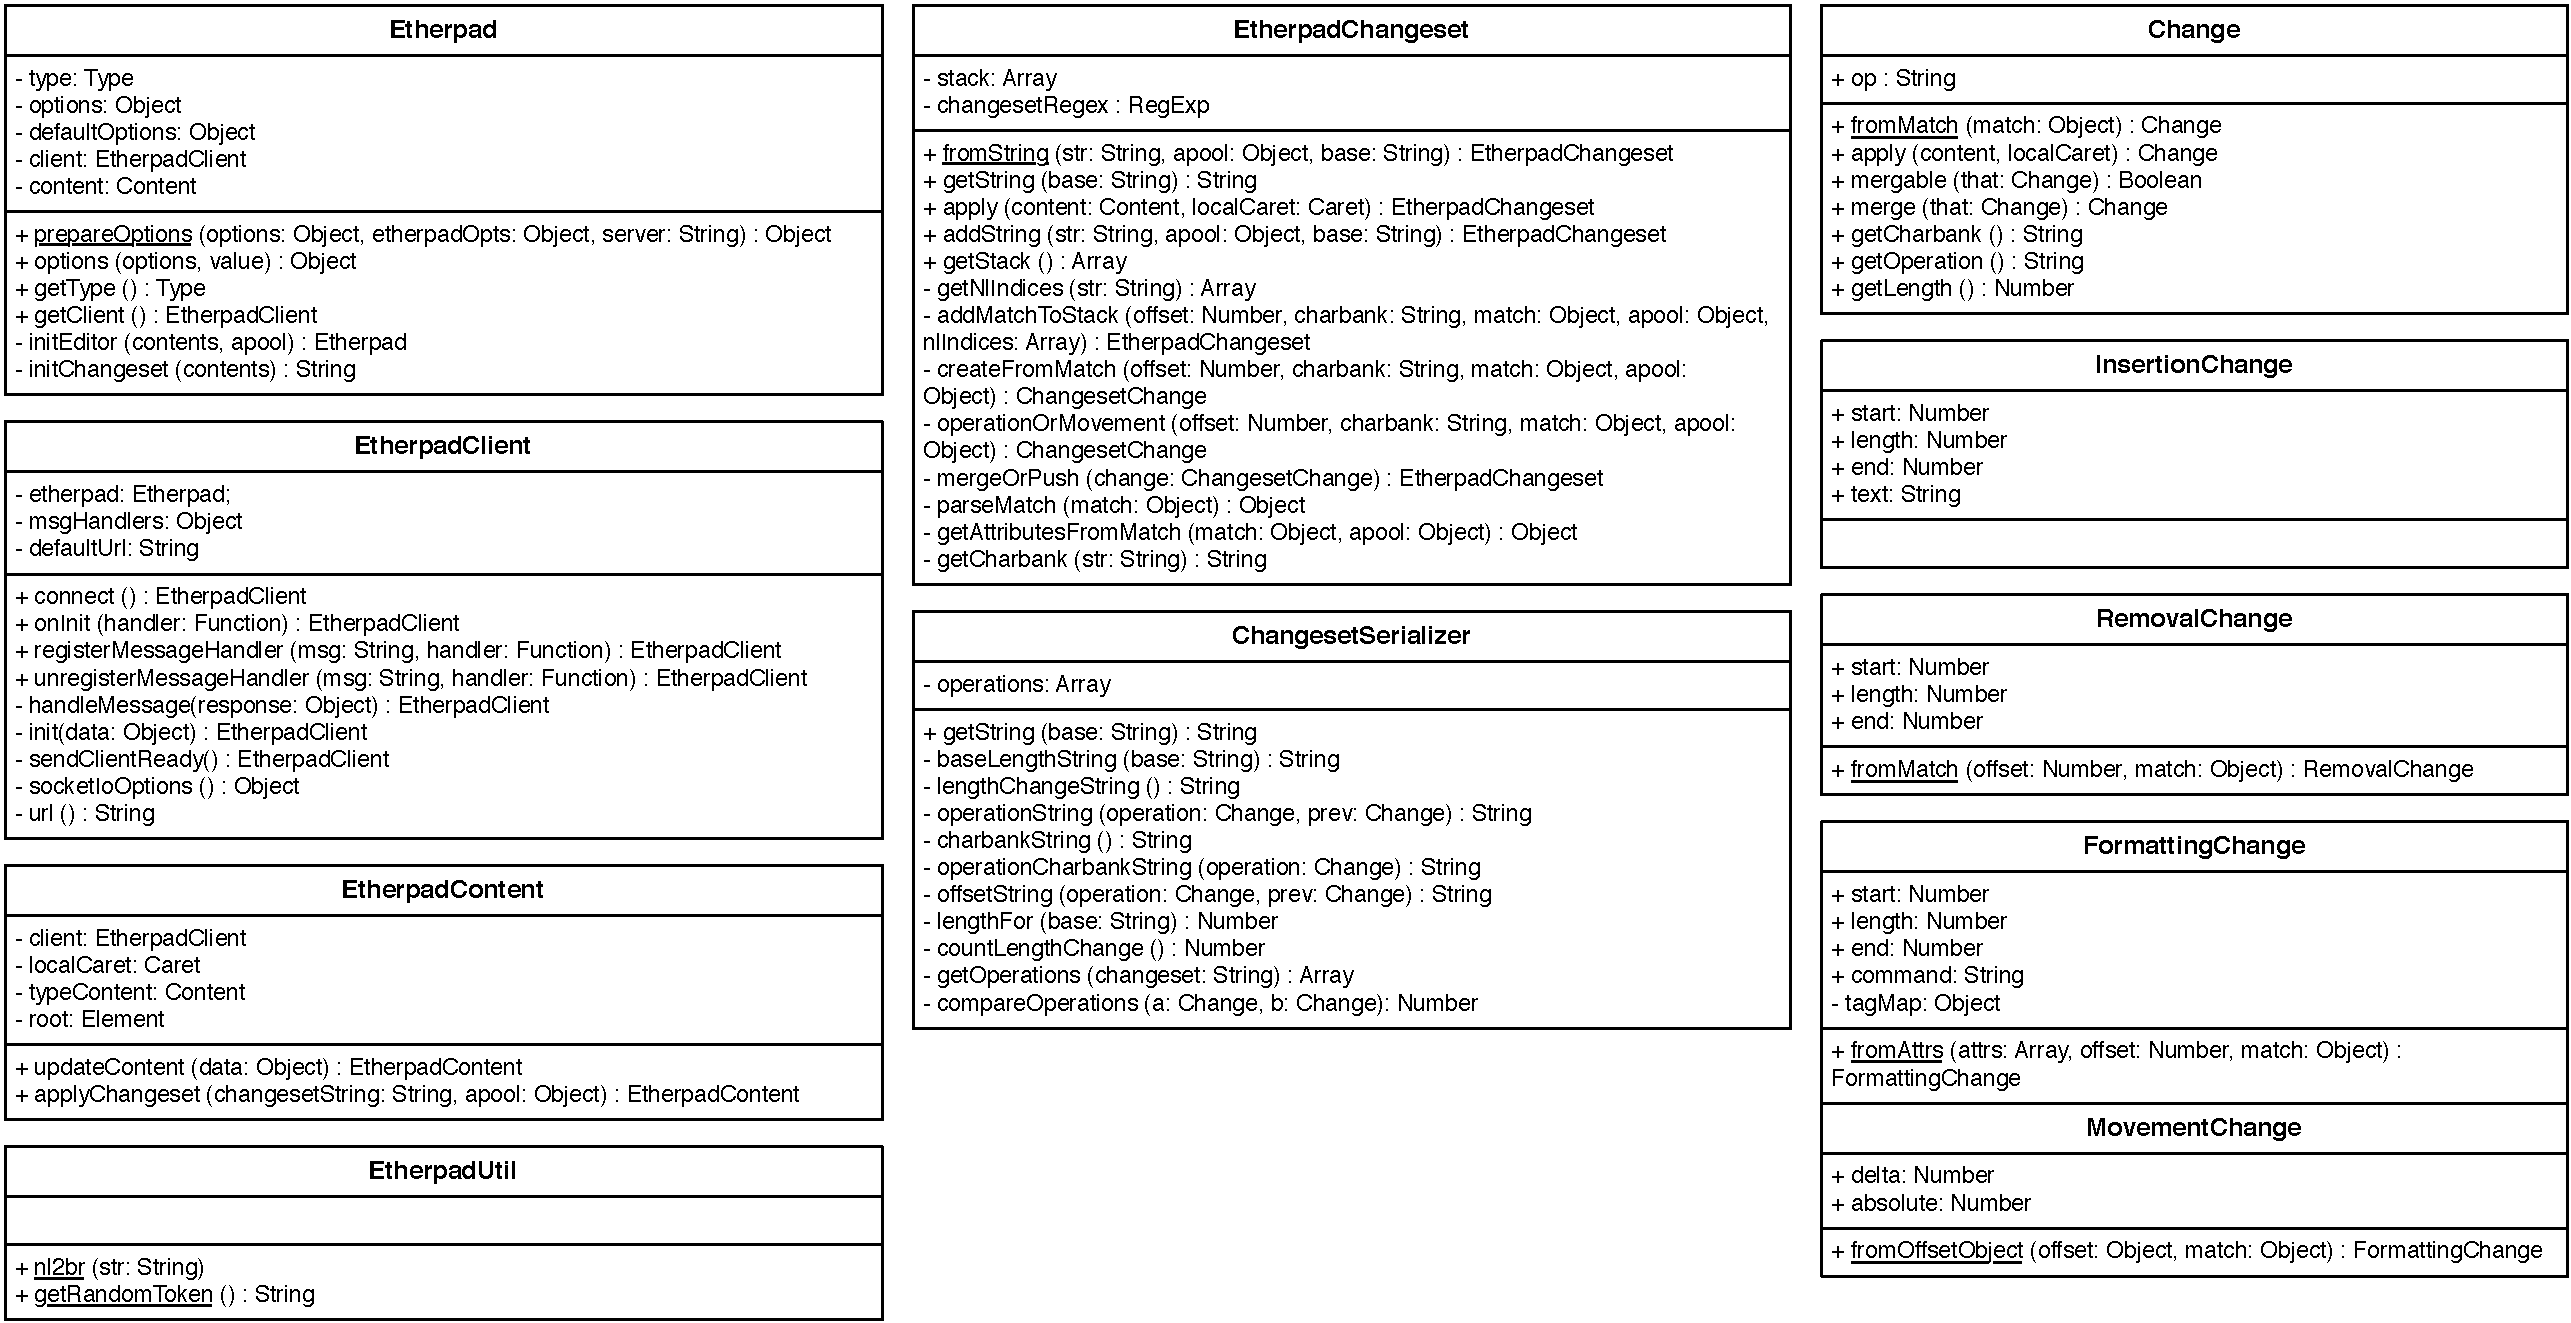
\includegraphics[width=\linewidth]{images/ClassesEtherpad}}
    \caption{Classes of the Etherpad Extension}
    \label{fig:classes_etherpad}
  \end{figure}
\end{landscape}

\clearpage
\newpage

